% -------------------------------------------------------------------------------------------------
% EVALUATION
% -------------------------------------------------------------------------------------------------
\section{Evaluation}
\label{sec:evaluation}
In this section, we will summarize the stages of the smart place life-cycle that already can be
automated with our solution. In our evaluation we will compare the software required to provisioning
the smart place infrastructure and also discuss about the advantages of our solution compared with
the others: full Virtual Machines and tools that implement the TOSCA standard.

\subsection{Preliminary Results}
\label{sub:preliminary_results}
As illustrated in Figure \ref{fig:smartplace_lifecycle} the smart place life-cycle is composed of several
stages. Our current prototype allows to automate some of these stages and our work in progress intend
to cover the remaining stages. Table \ref{table:summary} presents a summary of the smart place
life-cycle stages that our solution automates.
% Preliminary results table
\begin{table}[ht!]
    \centering
    \begin{tabular}{|c|c|c|c|}
    \hline
    Stage                     & In Progress & Completed   & Out of Scope \\ \hline
    Install Readers/Sensors   & ~           & ~           & X            \\ \hline
    Deploy Cloud Server       & ~           & X           & ~            \\ \hline
    Configure Readers/Sensors & X           & ~           & ~            \\ \hline
    Upload Events             & X           & ~           & ~            \\ \hline
    QoS Monitoring            & ~           & X           & ~            \\ \hline
    Undeploy                  & ~           & X           & ~            \\ \hline
    \end{tabular}
    \caption{Life-cycle automation summary.}
    \label{table:summary}
\end{table}

Our current prototype can automate the provisioning and deprovision the smart place
computing infrastructure. Regarding the \textit{QoS} monitoring, our solution leverages a service
available in AWS (CloudWatch), although we intend to perform the monitoring with a solution that
is independent of a particular provider. The remaining stages (reader/sensors configuration and event
upload) are in development - the automation of these stages will be available only for solutions
that are based on the Fosstrak platform.

\subsection{Container-based vs. VM-based solution}
\label{sub:container_vs_vm_solution}
We want our provisioned stack to be as small as possible, without the performance of our solution being
affected. The provisioning of the RFID software in Cloud4Things is performed through Docker containers.
A alternative to provisioning the RFID software stack is to use Virtual Machines. However, full VM presents
an overhead regarding the amount of resources that are consumed. In Figure \ref{fig:container_vs_vm}
we illustrate a comparison of the stacks between our solution and a full VM solution.

% Container vs. VM stack
\begin{figure}[!ht]
  \centering
  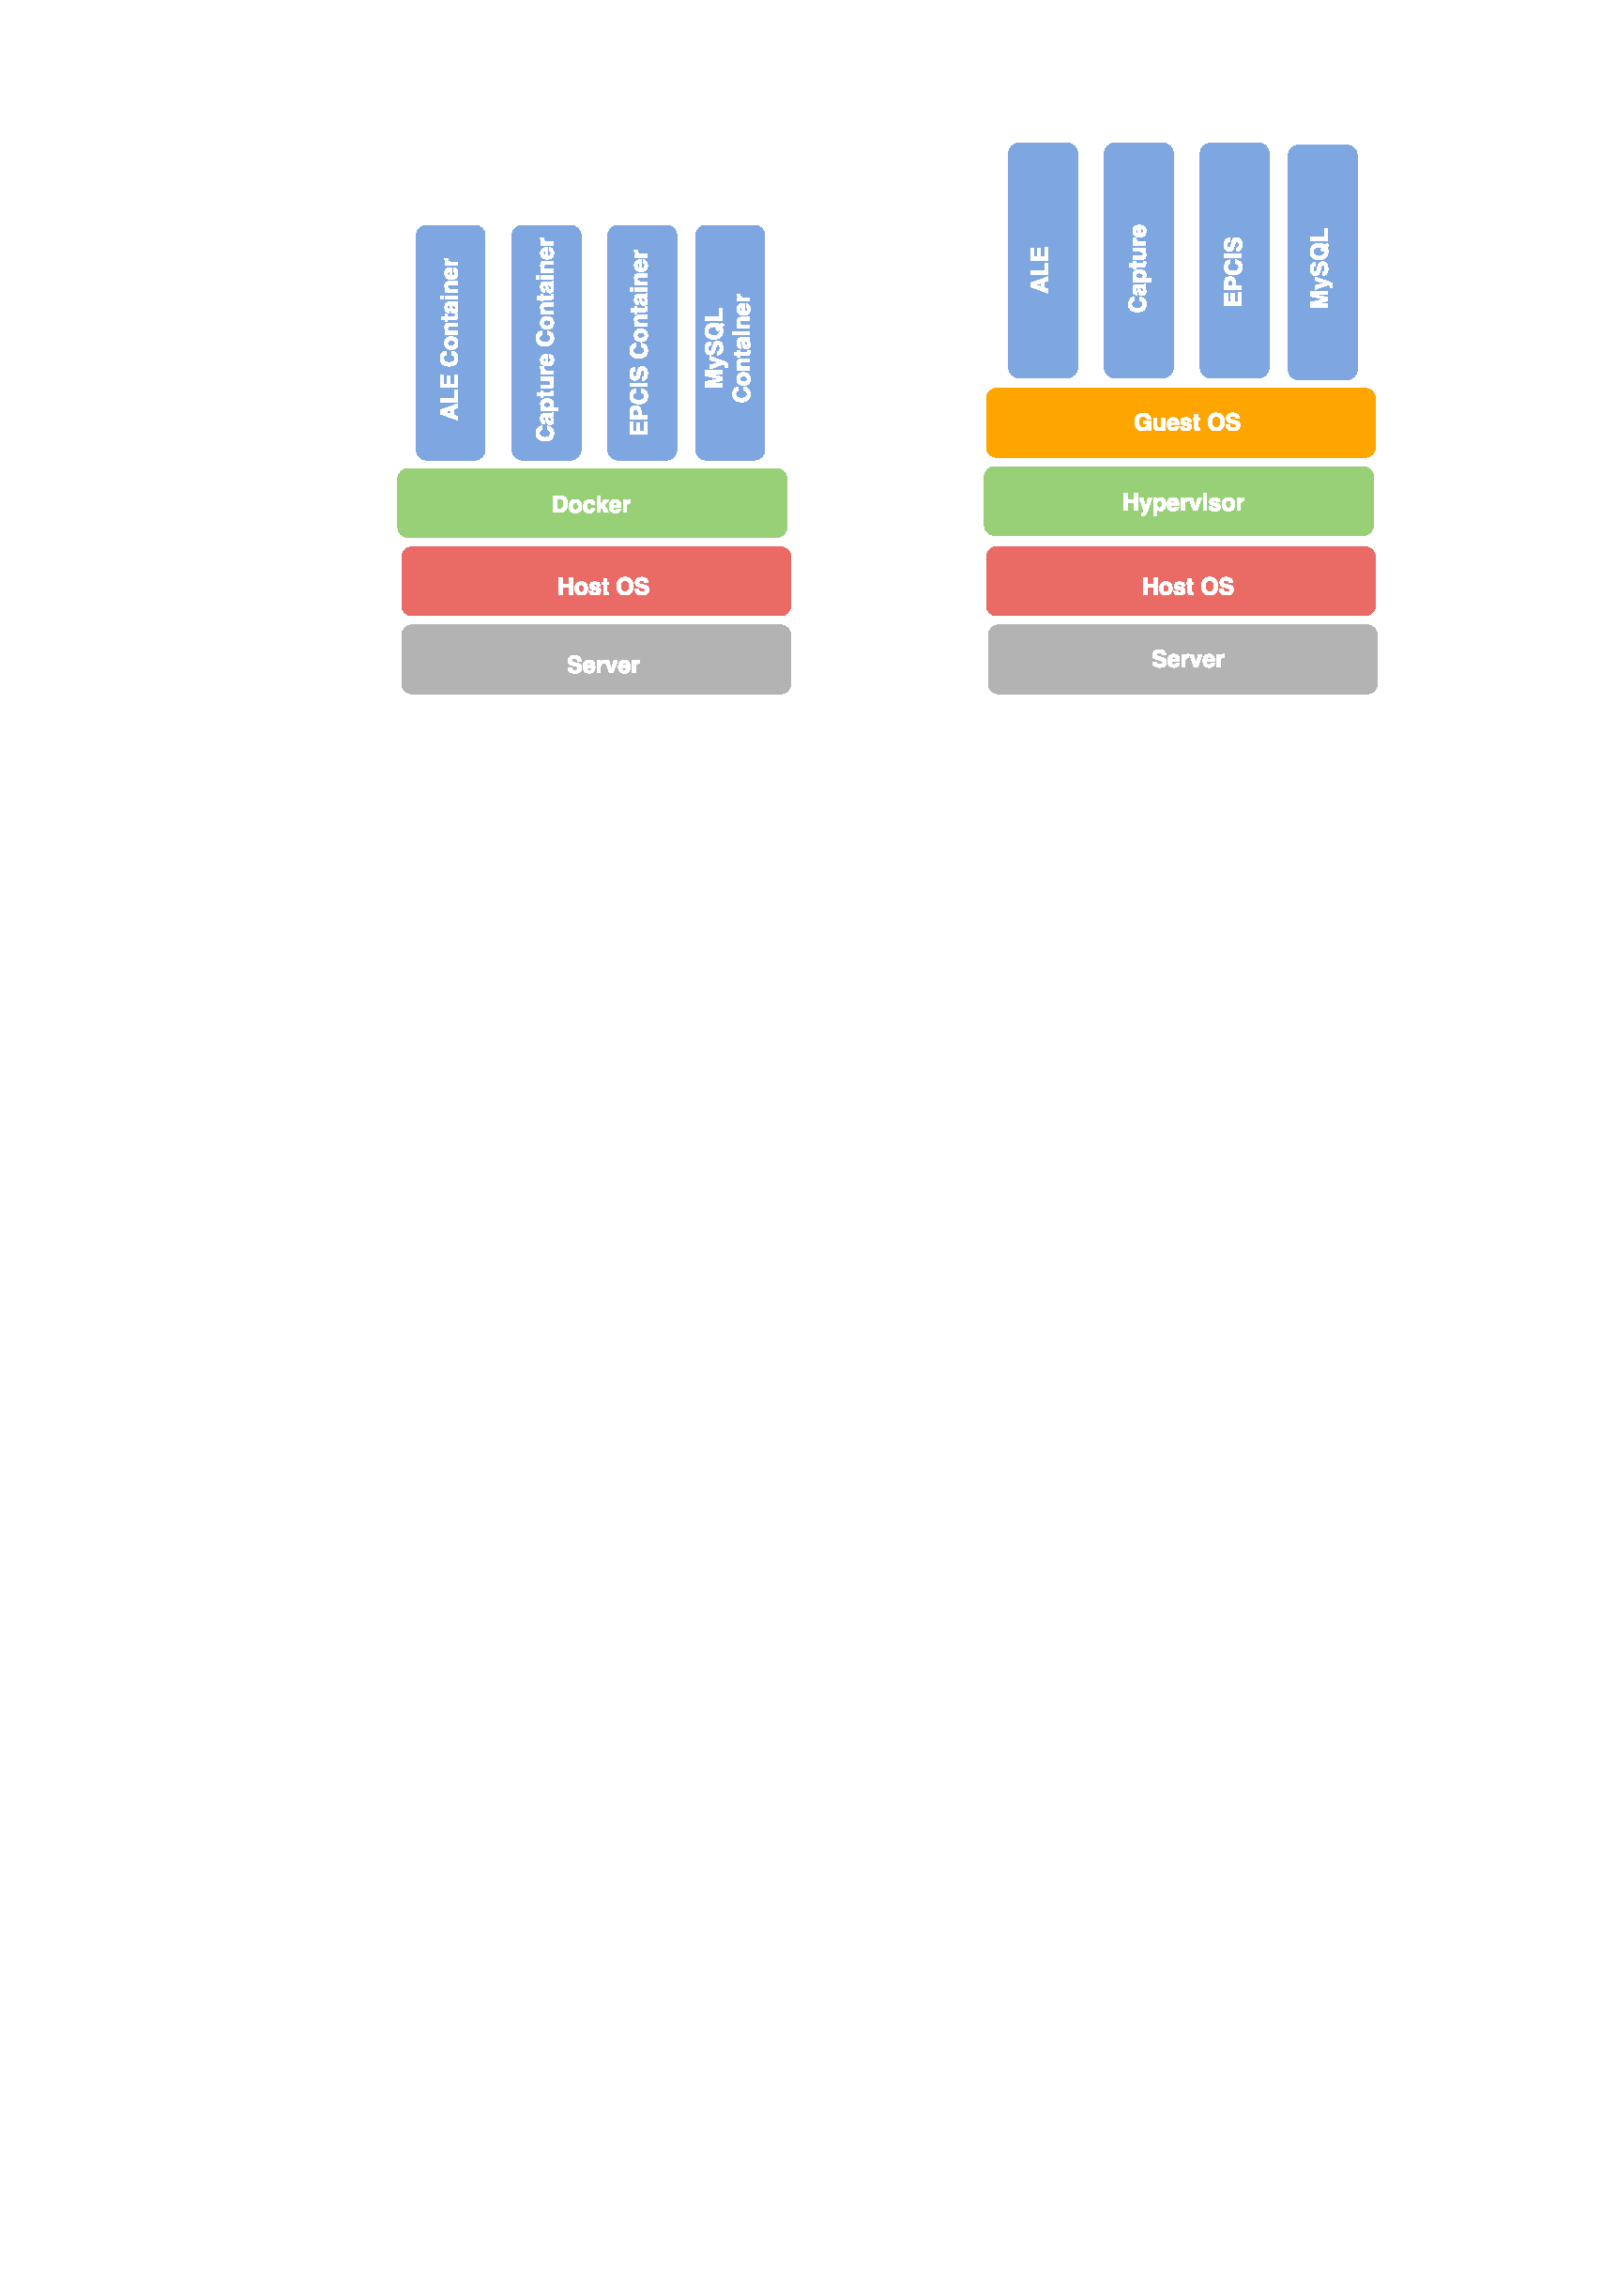
\includegraphics[width=.75\textwidth]{images/container-vs-vm-stack.pdf}
  \caption{Container vs. VM stack}
  \label{fig:container_vs_vm}
\end{figure}

The current implementation is running in a Amazon Linux based EC2 instance with a 8GB volume storage.
After provisioning the stack our implementation is using $\sim$2.6GB of the available storage, which $\sim$1.4GB
corresponding to the storage allocated by the Docker containers, as illustrated in Table \ref{table:containers_size}.

% Containers Size
\begin{table}[!ht]
\centering
\begin{tabular}{|c|c|}
\hline
\multicolumn{1}{|c|}{Container} & \multicolumn{1}{c|}{Size} \\ \hline
MySQL Database                  & 290 MB                    \\ \hline
EPCIS Repository                & 400 MB                    \\ \hline
Capture Application             & 381 MB                    \\ \hline
ALE Server                      & 390 MB                    \\ \hline
\end{tabular}
\caption{Docker containers size.}
\label{table:containers_size}
\end{table}

To compare our Docker-based approach with a full VM solution, we configured a Virtual Box VM running
Ubuntu 14.04 LTS with the software stack required to have a full installation of Fosstrak. Compared
with our implementation, a full VM approach requires almost twice the available storage - $\sim$4.7GB.

\subsection{Cloud4Things vs. TOSCA-based tools}
\label{sub:c4t_vs_tosca}
TOSCA is a powerful tool that allows to describe the internal topology and deployment process of cloud applications.
However, to provisioning the smart place infrastructure with TOSCA, a special provisioning engine for TOSCA is needed.
Currently there are several tools that implements a provisioning engine for TOSCA such as Ubuntu Juju\footnote{http://www.ubuntu.com/cloud/tools/juju},
Cloudify\footnote{http://getcloudify.org/} and the open-source implementation OpenTOSCA\footnote{http://www.iaas.uni-stuttgart.de/OpenTOSCA/}.

These tools allows the modeling of the application topology and deployment process in a more expressive way compared
to using only configuration management tools. Although TOSCA standard is very promising, is not fully developed yet
and does not support features that are used in our solution, such as container technologies.
